\documentclass[10pt,show notes on second screen]{beamer}

\usepackage{appendixnumberbeamer}
\usepackage[numbers,sort&compress]{natbib}
\usepackage{amsfonts}
\usepackage{amsmath}
\usepackage{mathtools}
\usepackage{amssymb}
\usepackage{mathrsfs}
\usepackage{units}

% For LatViz animations
\usepackage{animate}

% For nice algoritms
\usepackage{algorithm}
\usepackage{algorithmicx}
\usepackage{algpseudocode}

% For coloring equations
\usepackage{color}
\makeatletter
\def\mathcolor#1#{\@mathcolor{#1}}
\def\@mathcolor#1#2#3{%
\protect\leavevmode\begingroup\color#1{#2}#3\endgroup}
\makeatother

% % For proper referencing
\usepackage{varioref}
\usepackage{hyperref}
\hypersetup{
    breaklinks={true},
}
\usepackage{cleveref}

% For writing C++ in listings
\usepackage{listings}
\lstset{language=C++,
        basicstyle=\ttfamily,
        keywordstyle=\color{blue}\ttfamily,
        stringstyle=\color{red}\ttfamily,
        commentstyle=\color{green}\ttfamily,
        morecomment=[l][\color{magenta}]{\#}
}

% For including sub figures
\usepackage{subcaption}

% For nice tables
\usepackage{booktabs}

% For figures and graphics'n stuff
\usepackage{graphicx}
\usepackage{caption}

% \usetheme[progressbar=frametitle]{metropolis}
\usetheme{metropolis}

% For notes
\usepackage{pgfpages}
\setbeamertemplate{note page}[plain]
\setbeameroption{show notes on second screen=bottom}

\usefonttheme[onlymath]{serif}

% Titles, date, ect.
\title{Solving \texorpdfstring{$\SU(3)$}{SU3} Yang-Mills theory on the lattice: a calculation of selected gauge observables with gradient flow}
\date{\today}
\author{Hans Mathias Mamen Vege}
\institute{University of Oslo}

\bibliographystyle{plainnat}

% Loads command list
% For Feynman slashes
\usepackage{slashed}

\newcommand{\husk}[1]{\color{red}#1\color{black}}
\newcommand{\TODO}[1]{\color{red}#1\color{black}}
\newcommand{\expect}[1]{\left\langle{#1}\right\rangle}
\newcommand{\Tr}{\mathrm{Tr}}
\newcommand{\tr}{\mathrm{tr}}
\newcommand{\dd}{\mathrm{d}}
\newcommand{\e}{\mathrm{e}}
\newcommand{\SU}{\mathrm{SU}}
\newcommand{\conj}[1]{\overline{#1}}
\newcommand{\sign}{\mathrm{sign}}
\newcommand{\epsrnd}{\varepsilon_\mathrm{rnd}}

% For fermi units
\newcommand{\fm}{\mathrm{fm}}

% Complex number notation
\renewcommand{\Re}{\operatorname{Re}}
\renewcommand{\Im}{\operatorname{Im}}

% Commands for writing shorthand lattice operators
\newcommand{\MU}{\hat{\mu}}
\newcommand{\NU}{\hat{\nu}}

\renewcommand{\vec}[1]{\boldsymbol{\mathbf{#1}}}
% BEGIN COMMANDS FROM LATEX FOR PHYSICISTS
% http://www.dfcd.net/articles/latex/latex.html
\newcommand{\ket}[1]{\left| #1 \right\rangle} % for Dirac bras
\newcommand{\bra}[1]{\left\langle #1 \right|} % for Dirac kets
\newcommand{\bket}[1]{\right| #1 \right\rangle} % for Dirac bras
\newcommand{\bbra}[1]{\left\langle #1 \left|} % for Dirac kets

% Front page
\setbeamertemplate{title page}{
    \begin{minipage}[c][\paperheight]{\textwidth}
        \ifx\inserttitlegraphic\@empty\else\usebeamertemplate*{title graphic}\fi
        \vfill%
        {
        \centering
        \ifx\inserttitle\@empty\else\usebeamertemplate*{title}\fi
        \ifx\insertsubtitle\@empty\else\usebeamertemplate*{subtitle}\fi
        }
        \usebeamertemplate*{title separator}
        \begin{minipage}[t]{.4\textwidth}
            \ifx\beamer@shortauthor\@empty\else\usebeamertemplate*{author}\fi
            \ifx\insertdate\@empty\else\usebeamertemplate*{date}\fi
        \end{minipage}
        \begin{minipage}[t]{.6\textwidth}
            \vspace*{2em}
            {\hspace{1.2em}\small Supervisor: \textit{Andrea Shindler} \par}
            \vspace*{0.2em}
            {\hspace{1.2em}\small Co-supervisor: \textit{Morten Hjorth-Jensen}}
        \end{minipage}%

        \begin{minipage}[t]{\textwidth}
            \centering
            \ifx\insertinstitute\@empty\else\usebeamertemplate*{institute}\fi
        \end{minipage}
        \vfill
        \vspace*{1mm}
    \end{minipage}
}



\newcommand{\CC}{C\nolinebreak\hspace{-.05em}\raisebox{.4ex}{\tiny\bf +}\nolinebreak\hspace{-.10em}\raisebox{.4ex}{\tiny\bf +}}
\def\CC{{C\nolinebreak[4]\hspace{-.05em}\raisebox{.4ex}{\tiny\bf ++ }}}

% For aligned undersets
\usepackage{stackengine}
\def\stacktype{L}
\setstackgap{L}{1.2\normalbaselineskip}
\stackMath
\tabularnewline

\begin{document}

\setbeamercolor{background canvas}{bg=white}
\maketitle

% \begin{frame}{Structure}
%   % \setbeamertemplate{section in toc}[sections numbered]
%   \tableofcontents[hideallsubsections]
% \end{frame}

%%%%%%%%%%%%%%%%%%%%%%%%%%%%%%%%%%%%%%%%%%%%%%%%%%%%%%%%%%%%%%%%%%%%%%%%%%%%%%%%%%%%%%%%%%
%  ___       _                 _            _   _
% |_ _|_ __ | |_ _ __ ___   __| |_   _  ___| |_(_) ___  _ __
%  | || '_ \| __| '__/ _ \ / _` | | | |/ __| __| |/ _ \| '_ \
%  | || | | | |_| | | (_) | (_| | |_| | (__| |_| | (_) | | | |
% |___|_| |_|\__|_|  \___/ \__,_|\__,_|\___|\__|_|\___/|_| |_|
%%%%%%%%%%%%%%%%%%%%%%%%%%%%%%%%%%%%%%%%%%%%%%%%%%%%%%%%%%%%%%%%%%%%%%%%%%%%%%%%%%%%%%%%%%
\section{Introduction}

\begin{frame}{Structure}
    \begin{itemize}[<+->]
        \item Quantum Chromodynamics(QCD).
        \item Lattice QCD.
        \item Gradient flow.
        \item Developing a code for solving $\SU(3)$ Yang-Mills theory.
        \item Results.
    \end{itemize}
    \note{
    \begin{itemize}[<+->]
        \item \textbf{QCD.} We will go through and explain what QCD as well as motivate its existence.
        \item \textbf{LQCD.} We will briefly show how one discretise the lattice and perform calculations on it.
        \item \textbf{Gradient flow.} We will quickly introduce gradient flow and explain its effects.
        \item \textbf{GLAC.} Will briefly present the code which we developed as well as some benchmarks. We will also present the Metropolis algorithm.
        \item \textbf{Results.} We will present the results obtained from pure gauge calculations.
    \end{itemize}
    }
\end{frame}

%%%%%%%%%%%%%%%%%%%%%%%%%%%%%%%%%%%%%%%%%%%%%%%%%%%%%%%%%%%%%%%%%%%%%%%%%%%%%%%%%%%%%%%%%%
%   ___   ____ ____
%  / _ \ / ___|  _ \
% | | | | |   | | | |
% | |_| | |___| |_| |
%  \__\_\\____|____/
%%%%%%%%%%%%%%%%%%%%%%%%%%%%%%%%%%%%%%%%%%%%%%%%%%%%%%%%%%%%%%%%%%%%%%%%%%%%%%%%%%%%%%%%%%
\section{Quantum Chromodynamics(QCD)}

\begin{frame}{QCD}
\begin{itemize}[<+->]
    \item The standard model: Six quarks and eight gluons
    \item Asymptotic freedom
    \item Confinement
    \item Highly nonlinear due to gluon self-interactions
\end{itemize}
\note{
\begin{itemize}[<+->]
    \item \textbf{The standard model.} 
    \item \textbf{Asymptotic freedom.} 
    \item \textbf{Confinement.} 
    \item \textbf{Nonlinearity.} 
\end{itemize}
}
\end{frame}

\begin{frame}{The Standard Model}
    \begin{center}
        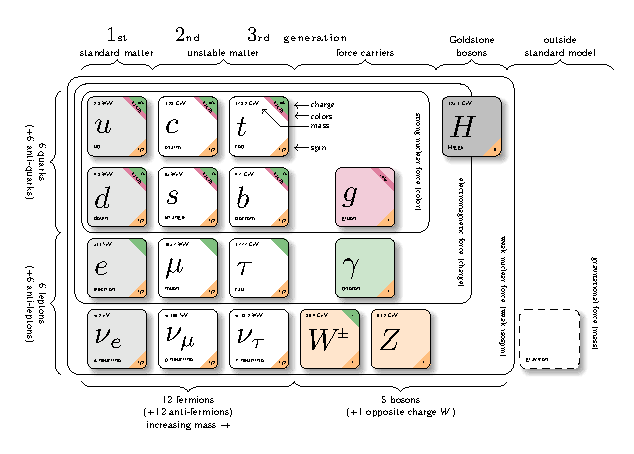
\includegraphics[width=0.8\textwidth]{../figures/illustrations/qcd/standard-model/sm.pdf}
    \end{center}
    \note{Consists of the innermost square of the six quarks and the gluons.}
\end{frame}

\begin{frame}{Asymptotic freedom}
    \begin{center}
        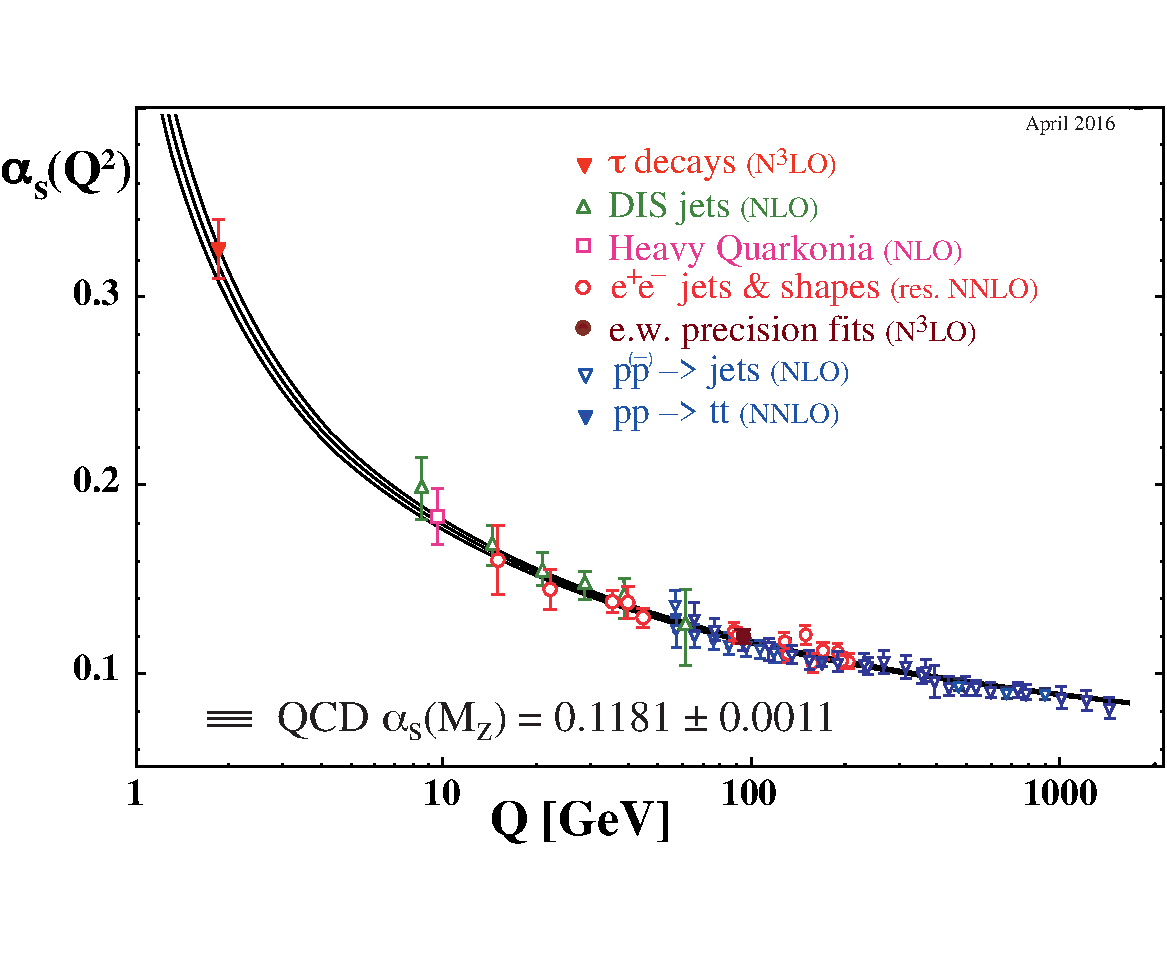
\includegraphics[width=0.8\textwidth]{../figures/pdg_asymptotic_freedom-eps-converted-to.pdf}
    \end{center}
    \note{
        \begin{itemize}
            \item The coupling constant \textbf{decreases} as we \textbf{increase} the energy
            \item One of the experimental proofs of QCD along with triple $\gamma$ decay and muon cross section ration $R$.
        \end{itemize}
    }
\end{frame}

\begin{frame}{Confinement}
    \begin{center}
        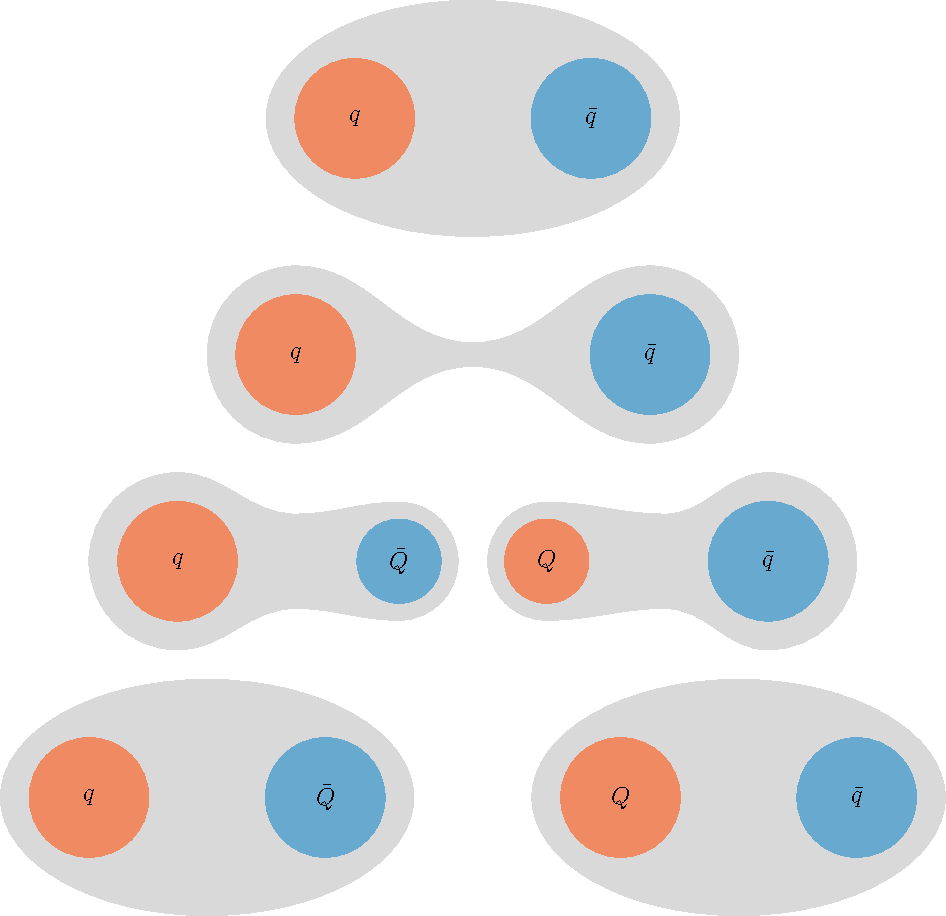
\includegraphics[width=0.65\textwidth]{../figures/illustrations/qcd/confinement/string-breaking.pdf}
    \end{center}
    \note{If we try to pull apart \textbf{two mesons}, more and more energy is required until we have enough energy to spontaneously create a \textbf{quark-antiquark} pair, forming thus \textbf{two new mesons.}}
\end{frame}

\begin{frame}{The non-linearity of QCD}
The QCD Lagrangian
\begin{align*}
    \mathcal{L}_\mathrm{QCD} = \sum^{N_f}_{f=1} \bar{\psi}^{(f)} \left(i\slashed{D} - m^{(f)}\right) \psi^{(f)} - \frac{1}{4}G^a_{\mu\nu}G^{a\mu\nu},
\end{align*}
with action
\begin{align}
    S = \int \dd^4 x \mathcal{L}_\mathrm{QCD}.
\end{align}

\begin{align*}
    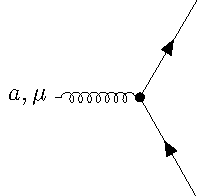
\includegraphics[scale=0.9]{../figures/feynman-diagrams/fermion-gluon-vertex/fermion-gluon-vertex.pdf} \quad
    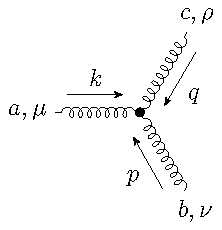
\includegraphics[scale=0.9]{../figures/feynman-diagrams/three-gluon-vertex/three-gluon-vertex.pdf} \quad
    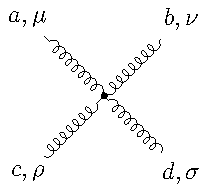
\includegraphics[scale=0.9]{../figures/feynman-diagrams/four-gluon-vertex/four-gluon-vertex.pdf}
\end{align*}
\end{frame}

\begin{frame}{Topology in QCD}
\begin{itemize}
    \item <1->Instantons
    \item <2->Topological charge, $Q$
    \item <3->Winding number
\end{itemize}

\begin{block}
\only<3->\begin{figure}
    \centering
    \begin{subfigure}{0.22\textwidth}
        \centering
        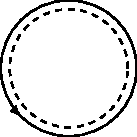
\includegraphics{../figures/illustrations/qcd/winding-number/winding-number1.pdf}
        \caption{$\nu=+1$}
    \end{subfigure}
    \begin{subfigure}{0.22\textwidth}
        \centering
        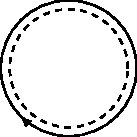
\includegraphics{../figures/illustrations/qcd/winding-number/winding-number-1.pdf}
        \caption{$\nu=-1$}
    \end{subfigure}
    \begin{subfigure}{0.22\textwidth}
        \centering
        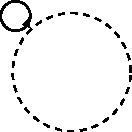
\includegraphics{../figures/illustrations/qcd/winding-number/winding-number0.pdf}
        \caption{$\nu=0$}
    \end{subfigure}
    \begin{subfigure}{0.22\textwidth}
        \centering
        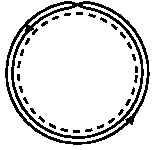
\includegraphics{../figures/illustrations/qcd/winding-number/winding-number+2.pdf}
        \caption{$\nu=+2$}
    \end{subfigure}
    \caption{The figure is taken from \citet[p. 32]{forkel_primer_2000}.}
\end{figure}
\end{block}
\note{
    \begin{itemize}
        \item <1->\textbf{Instantons} are local minimums to the Yang-Mills action in Euclidean space.
        \item <2->Measuring \textbf{topological charge} is a measure of the \textit{Winding number} of the gauge field.
        \item <3->An illustration of how one can view the winding number given a function $f$ that parametrizes a path around a circle $S^1$. Given that it starts and ends at the same point, we have that the number of times it wraps around the circle gives us the winding number.
    \end{itemize}
}

\end{frame}

\begin{frame}{The Witten-Veneziano relation}
A formula connecting pure gauge theory and full QCD.
\begin{align}
    m_{\eta'}^2 = \frac{2N_f}{f^2_\pi}\chi_\mathrm{top}
\end{align}
\begin{itemize}
    \item Pion decay constant $f_\pi=0.130(5)/\sqrt{2}$ GeV.
    \item $\eta'$ meson mass $m_{\eta'}=0.95778(6)$ GeV.
    \item $\chi_\mathrm{top}$ is the \textit{topological susceptibility}.
\end{itemize}
\note{
    \begin{itemize}
        \item We use the experimental values for the pion decay constant and the $\eta'$ mass.
        \item Allows us to estimate the number of flavors in our theory $N_f$.
        \item $\chi_\mathrm{top}$ is the topological susceptibility, calculated from the expectation value of $Q$.
    \end{itemize}
}
\end{frame}

%%%%%%%%%%%%%%%%%%%%%%%%%%%%%%%%%%%%%%%%%%%%%%%%%%%%%%%%%%%%%%%%%%%%%%%%%%%%%%%%%%%%%%%%%%
%  _          _   _   _             ___   ____ ____
% | |    __ _| |_| |_(_) ___ ___   / _ \ / ___|  _ \
% | |   / _` | __| __| |/ __/ _ \ | | | | |   | | | |
% | |__| (_| | |_| |_| | (_|  __/ | |_| | |___| |_| |
% |_____\__,_|\__|\__|_|\___\___|  \__\_\\____|____/
%%%%%%%%%%%%%%%%%%%%%%%%%%%%%%%%%%%%%%%%%%%%%%%%%%%%%%%%%%%%%%%%%%%%%%%%%%%%%%%%%%%%%%%%%%
\section{Lattice Quantum Chromodynamics(LQCD)}

\begin{frame}{Discretizing spacetime}
\begin{enumerate}[<+->]
    \item Divide spacetime into a cube of size $N^3\times N_T$.
    \item Fermions live on the each \textit{point} in the cube.
    \item The gauge fields live on the sites \textit{in between} the points, and is called links.
\end{enumerate}
\end{frame}

\begin{frame}{Links}
A link
\begin{align*}
    U_\mu(n) = \exp \left[ i a A_\mu (n) \right],
\end{align*}
connects one lattice site to another and is a $\SU(3)$ matrix.
\begin{figure}
    \centering
    \begin{subfigure}{0.48\textwidth}
        \centering
        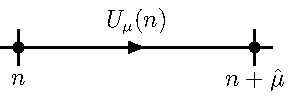
\includegraphics{../figures/illustrations/lqcd/links/link}
        \label{fig:lqcd:link}
    \end{subfigure}
    \begin{subfigure}{0.48\textwidth}
        \centering
        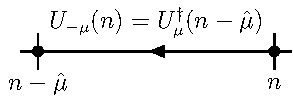
\includegraphics{../figures/illustrations/lqcd/links/link-inverse}
        \label{fig:lqcd:link-inverse}
    \end{subfigure}
    \centering
\end{figure}
where $U_{-\mu}(n) = U_\mu(n - \hat{\mu})^\dagger$.

\note{
    \begin{itemize}
        \item Defined from the gauge transporter.
        \item A link in the positive $\MU$ direction is shown in the figure to the left.
        \item A link in the negative $\MU$ direction is shown in the figure to the right.
    \end{itemize}
}
\end{frame}

\begin{frame}{Gauge invariance on the lattice}
\begin{block}
    \only<1->{Links gauge transform as}
    \only<1->{\begin{align*}
            U_\mu(n) &\rightarrow U_\mu'(n) = \Omega(n) U_\mu(n) \Omega(n+\hat{\mu})^\dagger, \\
            U_{-\mu}(n) &\rightarrow U_{-\mu}'(n) = \Omega(n) U_{\mu}(n-\hat{\mu})^\dagger \Omega(n-\hat{\mu})^\dagger.
        \end{align*}}
    \only<2->{Two main types of gauge invariant objects,}
    \begin{itemize}
        \item<3-> Fully connected gauge invariant objects.
        \item<3-> Objects with fermions $\psi$, $\bar{\psi}$ as end points.
    \end{itemize}
\end{block}
\end{frame}

\begin{frame}{The plaquette}
The simplest gauge invariant object,
\begin{align*}
    P_{\mu\nu}(n) &= U_\mu(n) U_{\nu}(n+\hat{\mu}) U_{-\mu}(n+\hat{\mu}+\hat{\nu}) U_{-\nu} (n+\hat{\nu}) \nonumber \\
    &= U_\mu(n) U_{\nu}(n+\hat{\mu}) U_{\mu}(n+\hat{\nu})^\dagger U_{\nu} (n)^\dagger,
\end{align*}
\begin{figure}
    \centering
    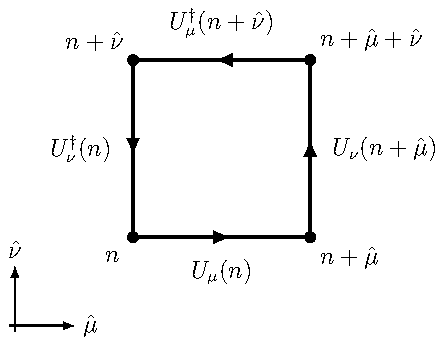
\includegraphics[scale=1]{../figures/illustrations/lqcd/plaquette/plaquette}
\end{figure}
\end{frame}

\begin{frame}{The Wilson gauge action}
The Wilson gauge action is given as
\begin{align}
    S_G[U] = \frac{\beta}{3} \sum_{n\in\Lambda} \sum_{\mu<\nu} \Re \tr \left[ 1 - P_{\mu\nu}(n) \right],
\end{align}
with $\beta=6/g_S^2$.
\note{
    \begin{itemize}
        \item Using the definition of the link we saw earlier, we can reproduce the continuum action up to an discretization error of $\mathcal{O}(a^2)$.
    \end{itemize}
}
\end{frame}

%%%%%%%%%%%%%%%%%%%%%%%%%%%%%%%%%%%%%%%%%%%%%%%%%%%%%%%%%%%%%%%%%%%%%%%%%%%%%%%%%%%%%%%%%%
%  ____                 _             _                                     _
% |  _ \  _____   _____| | ___  _ __ (_)_ __   __ _    __ _    ___ ___   __| | ___
% | | | |/ _ \ \ / / _ \ |/ _ \| '_ \| | '_ \ / _` |  / _` |  / __/ _ \ / _` |/ _ \
% | |_| |  __/\ V /  __/ | (_) | |_) | | | | | (_| | | (_| | | (_| (_) | (_| |  __/
% |____/ \___| \_/ \___|_|\___/| .__/|_|_| |_|\__, |  \__,_|  \___\___/ \__,_|\___|
%                              |_|            |___/
%%%%%%%%%%%%%%%%%%%%%%%%%%%%%%%%%%%%%%%%%%%%%%%%%%%%%%%%%%%%%%%%%%%%%%%%%%%%%%%%%%%%%%%%%%
\section{Developing a code for solving \texorpdfstring{$\SU(3)$}{SU3} Yang-Mills theory on the lattice}

\begin{frame}{The numerical challenge in lattice QCD}
\onslide<1->{A lattice configuration consists of $\SU(3)$ matrices,}
\onslide<2->{\begin{align*}
    \stackunder{\underbrace{N^3}}{\text{Spatial}} \times \stackunder{\underbrace{N_T}}{\text{Temporal}} \times \stackunder{\underbrace{4}}{\text{Links}} \times \stackunder{\underbrace{9}}{\text{$\SU(3)$ matrix}} \times \stackunder{\underbrace{2}}{\text{$\mathbb{C}$-numbers}} = 72 N^3N_T,
\end{align*}}
\onslide<3->{$\rightarrow 8 \times 72N^3N_T$ bytes.}
\note{
    \begin{itemize}
        \item The $\SU(3)$ matrices are $3\times 3$ matrices of nine complex numbers or 18 real numbers.
        \item This leads to an absolute \textbf{requirement of efficiency}, both in \textbf{calculations} and in \textbf{input/output}.
        \item When returning to what ensembles of configurations we generated this will be evident.
    \end{itemize}
}
\end{frame}

\begin{frame}{The path integral I}
\only<1>{\begin{align*}
    \langle O \rangle = \frac{1}{Z} \int \mathcal{D}U O[\psi,\bar{\psi},U] \e^{- S_G[U] - S_F[\psi,\bar{\psi},U]}.
\end{align*}}%
\only<2>{\begin{align*}
    \langle O \rangle = \frac{1}{Z} \int \mathcal{D}U O[U] \e^{- S_G[U]}.
\end{align*}}%
\only<3>{\begin{align*}
    \langle O \rangle = \mathcolor{red}{\frac{1}{Z}\int\mathcal{D}U} O[U] \mathcolor{red}{\e^{- S_G[U]}}.
\end{align*}}%
with 
\only<1>{\begin{align*}
Z = \int \mathcal{D}U \mathcal{D}\bar{\psi} \mathcal{D}\psi e^{- S_G[U] - S_F[\psi,\bar{\psi}, U]}.
\end{align*}}%
\only<2->{\begin{align*}
Z = \int \mathcal{D}U e^{- S_G[U]}.
\end{align*}}%
\end{frame}

\begin{frame}{The path integral II}
\begin{figure}
    \centering
    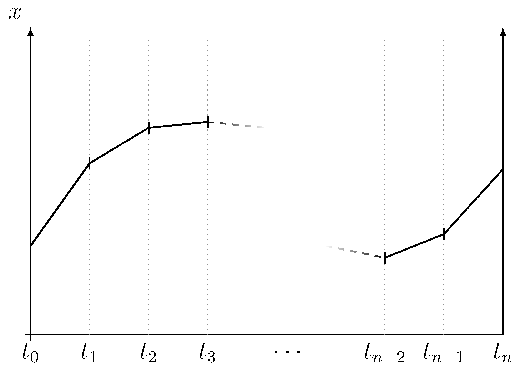
\includegraphics[scale=1.0]{../figures/illustrations/lqcd/path-integral/path-integral-flattened}
\end{figure}
\note{An example of the discretized path integral, going from time $t_0$ to $t_{N_T}$, where the end points is taken to be equal, $x_0=x_{N_T}$. We integrate over all of space at each time $t_i$ finding the most likely position at a given time.}
\end{frame}

\begin{frame}{How to measure}
The observable becomes an average over the $N_\mathrm{MC}$ gauge configurations.
\begin{align*}
    \expect{O} = \underset{N_\mathrm{MC}\rightarrow\infty}{\lim} \frac{1}{N_\mathrm{MC}} \sum^{N_\mathrm{MC}}_i O[U_i]
\end{align*}
\onslide<1->We now need to generate configurations...
\note{
\begin{itemize}
    \item We perform an average of the created configurations.
\end{itemize}
}
\end{frame}

\begin{frame}{The Metropolis algorithm}
\begin{algorithmic}
    \Repeat
        \State Randomly generate a candidate state $j$ with probability $T_{i\rightarrow i}$.
        \State Calculate $A_{i\rightarrow j}$ which saw on previous slide.
        \State Generate random number $u\in[0,1]$.
        \If {$u \leq A_{i\rightarrow j}$}
            \State Accept new state $j$.
        \ElsIf {$u > A_{i\rightarrow j}$}
            \State Reject new state $j$ and retain the old state $i$.
        \EndIf
    \Until {$N_\mathrm{MC}$ samples are generated.}
\end{algorithmic}
\note{
\begin{itemize}
    \item Generated state $j$ is a gauge configuration.
    \item Algorithm of choice when sampling gauge configurations.
    \item For generating $N_\mathrm{MC}$ Monte Carlo samples.
\end{itemize}
}
\end{frame}

\begin{frame}{The Metropolis algorithm on the lattice}
A parameter $\epsilon_\mathrm{rnd}$ controls the spread of the candidate matrices.
\begin{enumerate}
    \item Initialize lattice with $\SU(3)$ matrices close to unity(\textit{hot start}) or at unity(\textit{cold start}).
    \item Thermalize with $N_\mathrm{therm}$ sweeps.
    \item Generate $N_\mathrm{MC}$ samples,
    \begin{enumerate}[i]
        \item Perform $N_\mathrm{corr}$ correlation updates.
        \item At each update, perform $N_\mathrm{up}$ single link update for every lattice link.
        \item Store configuration and/or apply gradient flow and sample observables on it.
    \end{enumerate}
\end{enumerate}
\note{
\begin{itemize}
    \item We use \textbf{periodic boundary conditions} for all calculations.
    \item $N_\mathrm{MC}$ is how many configurations we will generate.
    \item $N_\mathrm{up}$ is how many single link updates we will perform.
    \item $N_\mathrm{corr}$ is how many full sweeps we shall perform in between each sampling. Needed in order to reduce the autocorrelation between the configurations.
\end{itemize}
}
\end{frame}

\begin{frame}{Parallelization}
Two methods used:
\begin{itemize}
    \item Single link sharing used in the Metropolis algorithm.
    \item \textit{shifts} used in in gradient flow and observable sampling
\end{itemize}
\note{
\begin{itemize}
    \item Tested out \textbf{halos}, but turned out to be problematic when generating.
    \item We parallelized using MPI.
\end{itemize}
}
\end{frame}

\begin{frame}{Shifts}
\begin{figure}
    \centering
    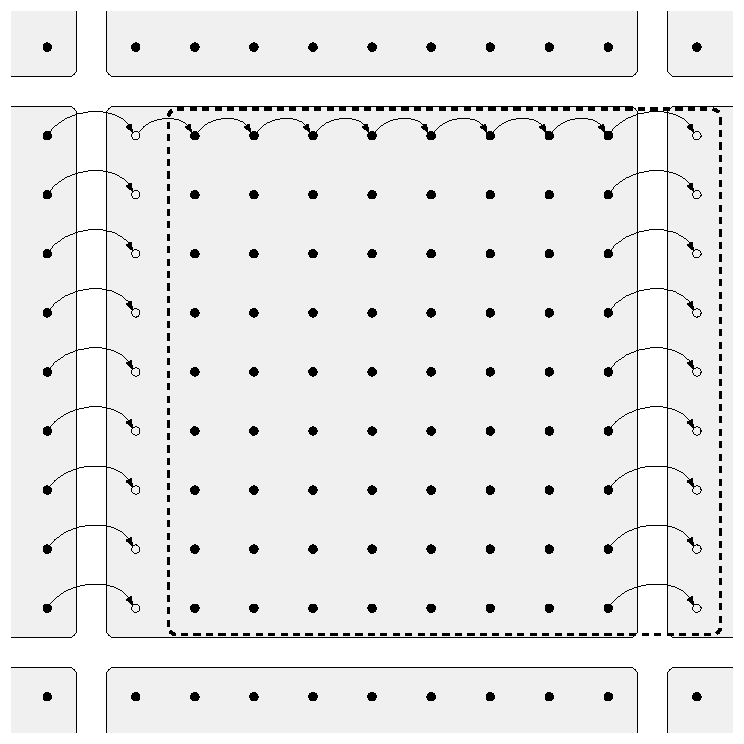
\includegraphics[scale=0.6]{../figures/illustrations/implementation/shift/shift}
\end{figure}
\note{
\begin{itemize}
    \item An illustration of the lattice shift. 
    \item The links $U_\nu$ of the lattice are copied over to a temporary lattice shifted in direction $\hat{\mu}$. 
    \item The face that is shifted over to an adjacent sub-lattice is shared through a non-blocking MPI call, while we copy the links to the temporary lattice.
    \item Allows for a simplified syntax close to that of the equations we are working with.
    \item Don't have to write out any loops over the lattice positions.
\end{itemize}
}
\end{frame}

\begin{frame}{Scaling}
We checked three types of scaling,
\begin{itemize}[<+->]
    \item \textbf{Strong scaling:} \textit{fixed problem} and a \textit{variable} $N_p$ \textit{cores}
    \item \textbf{Weak scaling:} \textit{fixed problem per processor} and a \textit{variable} $N_p$ \textit{cores}.
    \item \textbf{Speedup:} defined as $S(p) = \frac{t_{N_{p,0}}}{t_{N_p}}$.
\end{itemize}
\only<1>{\begin{center}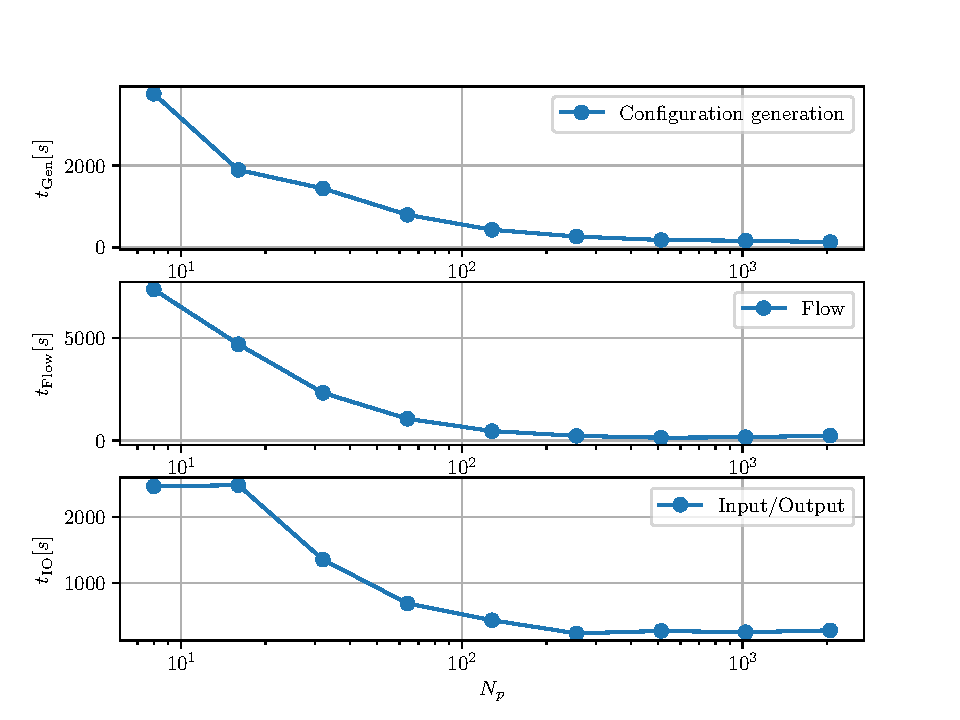
\includegraphics[trim={0.4cm 0.0cm 0.4cm 0.0cm},clip,scale=0.4]{../../LQCD/LatticeAnalyser/figures/scaling/strong/strong_all}\end{center}}
\only<2>{\begin{center}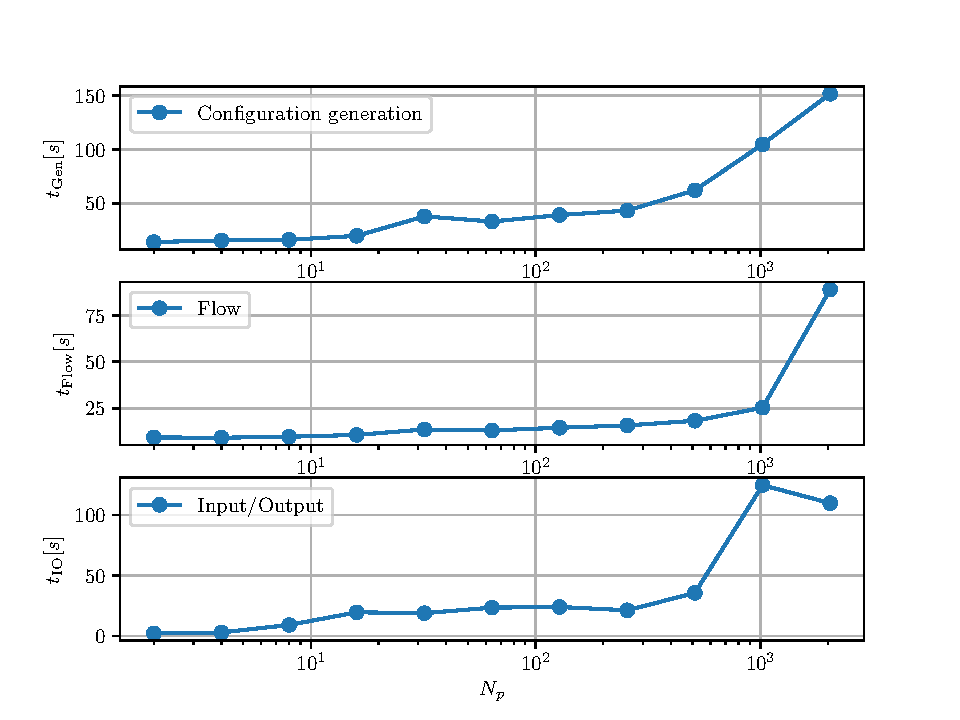
\includegraphics[trim={0.4cm 0.0cm 0.4cm 0.0cm},clip,scale=0.4]{../../LQCD/LatticeAnalyser/figures/scaling/weak/weak_all}\end{center}}
\only<3>{\begin{center}\includegraphics[trim={0.4cm 0.0cm 0.4cm 0.0cm},clip,scale=0.4]{../../LQCD/LatticeAnalyser/figures/scaling/strong/speedup_strong_all}\end{center}}
\note{
\begin{itemize}
\item <1->Strong scaling
\item <2->Weak scaling
\item <3->The speedup of the configuration generation, flowing, and IO. The speedup is calculated by dividing the run time of each $N_p$ run, with the run time of the run with the least number of processors, $N_p=8$.
\end{itemize}
\onslide<3->We appear to have a plateau around 512 cores.
}
\end{frame}

\begin{frame}{Optimizing the gauge configuration generation}
\only<1>{Generated 200 configurations for a lattice of size $N^3\times N_T = 16^3 \times 32$ and $\beta=6.0$, for combinations of $N_\mathrm{corr}\in[200,400,600]$ and $N_\mathrm{up}\in[10,20,30]$.}
\only<2>{\begin{center}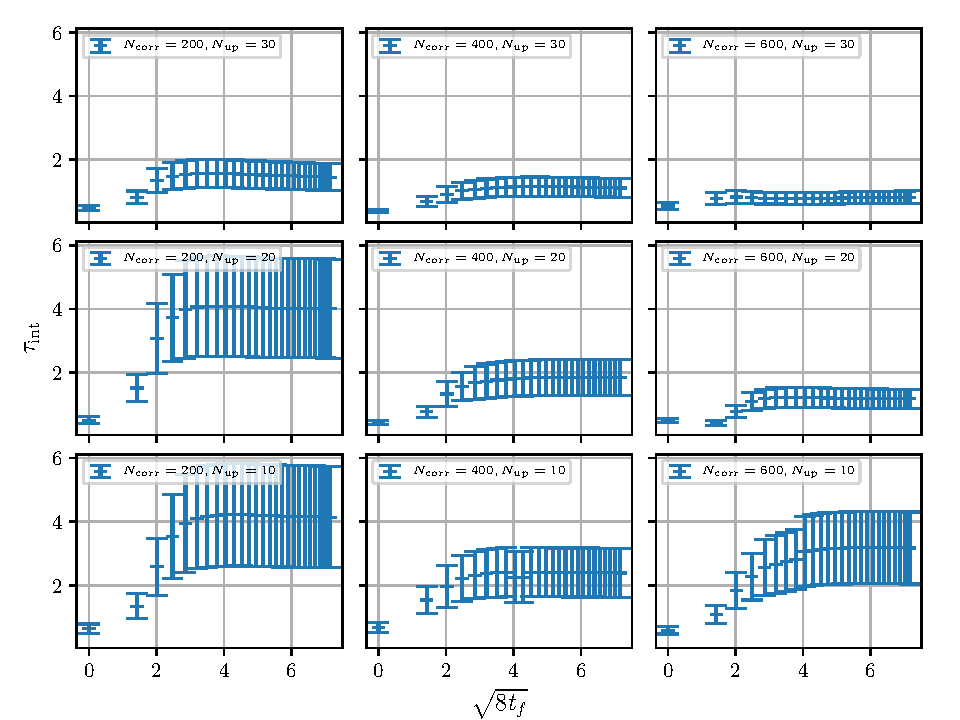
\includegraphics[trim={0.4cm 0.0cm 0.4cm 0.0cm},clip,scale=0.6]{../figures/lattice-updates/topc_autocorr}\end{center}}
\only<3>{\begin{center}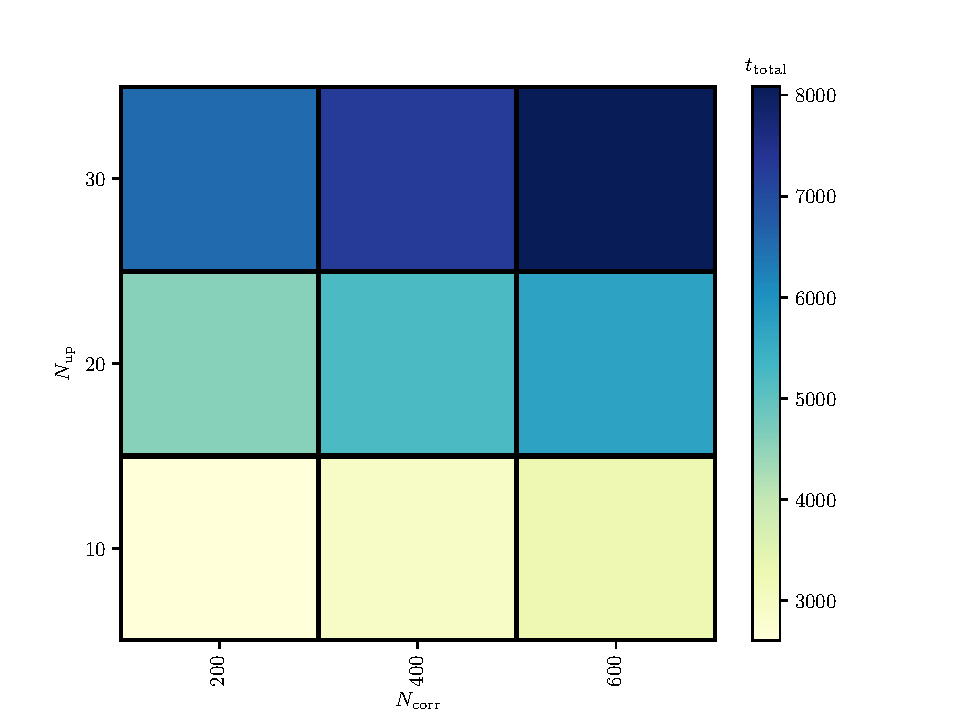
\includegraphics[trim={0.4cm 0.0cm 0.4cm 0.0cm},clip,scale=0.6]{../figures/lattice-updates/topc_total_runtime}\end{center}}
\note{
\begin{itemize}
    \item We run for different values for $N_\mathrm{up}$ and $N_\mathrm{corr}$ to see what gives optimizes \textbf{computational cost} and \textbf{autocorrelation}.
    \item <1> The integrated autocorrelation time for topological charge $\expect{Q}$ for a lattice of size $N=16$ and $N_T=32$ with $\beta=6.0$ for combinations of $N_\mathrm{corr}\in[200,400,600]$ and $N_\mathrm{up}\in[10,20,30]$, plotted against flow time $\sqrt{8t_f}$.
    \item <2> The time taking to generate 200 configurations and flowing them $N_\mathrm{flow}=250$ flow steps for a lattice of size $N=16$ and $N_T=32$, with $\beta=6.0$ for combinations of $N_\mathrm{corr}\in[200,400,600]$ and $N_\mathrm{up}\in[10,20,30]$.
\end{itemize}}
\end{frame}

%%%%%%%%%%%%%%%%%%%%%%%%%%%%%%%%%%%%%%%%%%%%%%%%%%%%%%%%%%%%%%%%%%%%%%%%%%%%%%%%%%%%%%%%%%
%   ____               _ _            _      __ _
%  / ___|_ __ __ _  __| (_) ___ _ __ | |_   / _| | _____      __
% | |  _| '__/ _` |/ _` | |/ _ \ '_ \| __| | |_| |/ _ \ \ /\ / /
% | |_| | | | (_| | (_| | |  __/ | | | |_  |  _| | (_) \ V  V /
%  \____|_|  \__,_|\__,_|_|\___|_| |_|\__| |_| |_|\___/ \_/\_/
%%%%%%%%%%%%%%%%%%%%%%%%%%%%%%%%%%%%%%%%%%%%%%%%%%%%%%%%%%%%%%%%%%%%%%%%%%%%%%%%%%%%%%%%%%
\section{Gradient flow}

\begin{frame}{The flow equation}
% Bad approx.: diffusion equation
% Topological charge preserved and is more pronounced 
% Why it is needed
% Certain quantities becomes renormalizable
The flow of the $\SU(3)$ gauge fields are denoted by $B_\mu(x,t_f)$ which are Lie algebra valued gauge fields,
\onslide<1->{\begin{align}
    \frac{\dd}{\dd t_f} B_\mu(x,t_f) = D_\nu G_{\nu\,\mu}(x,t_f), \label{eq:flow-continuum-diff-eq}
\end{align}}
\onslide<2->{\begin{align}
    D_\mu = \partial_\mu + \left[B_\mu(x,t_f), \cdot \right], \label{eq:flow-cont-covariant-derivative}
\end{align}}
\onslide<3->{\begin{align}
    G_{\mu\nu}(x,t_f) = \partial_\mu B_\nu(x,t_f) - \partial_\nu B_\mu(x,t_f) - i[B_\mu(x,t_f), B_\nu(x,t_f)], \label{eq:flow-field-strength-tensor}
\end{align}}
\onslide<4->{with the initial conditions being the fundamental gauge field,
\begin{align*}
    B_\mu(x,t_f)|_{t_f=0} = A_\mu(x).
\end{align*}}
\onslide<5->{
A bad approximation: \textit{the diffusion equation}, 
\begin{align*}
    \frac{\partial}{\partial t_f} B_\mu(x,t_f) \approx \partial^2 B_\mu(x,t_f)
\end{align*}
}
\onslide<6->{
    The smearing radius increases as $\sqrt{8t_f}$.
}
\note{
\begin{itemize}
    \item <1->The flow equation in the continuum is defined by this differential equation.
    \item <2->With the covariant derivative given by following, with the $\cdot$ being the derivative with respect to flow time.
    \item <3->The field strength tensor of the flown fields is given in the regular format.
    \item <4->The initial condition is the un-flowed gauge field, $A_\mu$.
    \item <5->Bad approx.: diffusion equation.
    \item <6->Topological charge preserved and is more pronounced.
    \item <6->Renormalizes the topological charge at non-zero flow time.
\end{itemize}
}
\end{frame}

\begin{frame}{Gradient flow on the lattice}
% RK3 classical and then on the lattice
\onslide<1->{\begin{align*}
    \dot{V}_{t_f}(x,\mu) = - g_S^2 \left\{\partial_{x,\mu} S_G[V_{t_f}] \right\} V_{t_f}(x,\mu),
\end{align*}}
\onslide<2->{with initial condition,
\begin{align*}
    V_{t_f}(x,\mu)|_{t_f=0} = U(x,\mu)
\end{align*}}
\onslide<3->{Note: need to find the action derivative $S_G[V_{t_f}]$.}
\note{
\begin{itemize}
    \item <1->On the lattice, the flow equation takes the shape in terms of the link variables.
    \item <2->Initial conditions similar to the continuum case.
    \item <3->The action derivative is also needed, but that is a minor task we will not cover here.
\end{itemize}
}
\end{frame}

\begin{frame}{Solving gradient flow with Runge-Kutta 3}
\onslide<1->{With
\begin{align*}
    \dot{V}_{t_f} = Z(V_{t_f}) V_{t_f} = - g_S^2 \left\{\partial_{x,\mu} S_G[V_{t_f}] \right\} V_{t_f},
\end{align*}}
\onslide<2->{we get
\begin{align*}
    \begin{split}
        &W_0 = V_{t_f}, \\
        &W_1 = \exp\left[\frac{1}{4}Z_0\right]W_0, \\
        &W_2 = \exp\left[\frac{8}{9}Z_1 - \frac{17}{36}Z_0\right]W_1, \\
        &V_{t_f + \epsilon_f} = \exp\left[\frac{3}{4}Z_2 - \frac{8}{9}Z_1 + \frac{17}{36}Z_0\right]W_2, \\
    \end{split}
\end{align*}
with coefficients from \citet{luscher_properties_2010}.}
\note{
\begin{itemize}
    \item <1-> We rewrite the equations slightly,
    \item <2-> and use a structure preserving integrator with coefficients from \citet{luscher_properties_2010}.
    \item <3-> We control the accuracy of this integrator by $\epsilon_f$.
\end{itemize}}
\end{frame}

\begin{frame}{Verifying the integration}
\only<1>{Testing the integrator for different integration steps $\epsilon_f$.
\begin{table}
    \centering
    \begin{tabular}{c c c c c c c c c c c}
    \toprule
    $\epsilon_f$ & $0.001$ & $0.005$ & $0.007$ & $0.009$ & $0.01$ & $0.02$ & $0.03$ & $0.05$ & $0.1$ & $0.5$ \\ \bottomrule
    \end{tabular}
\end{table}}
\only<2>{Lattice size $N^3\times N_T = 24^3 \times 48$ with $\beta=6.0$.
\begin{figure}
    \centering
    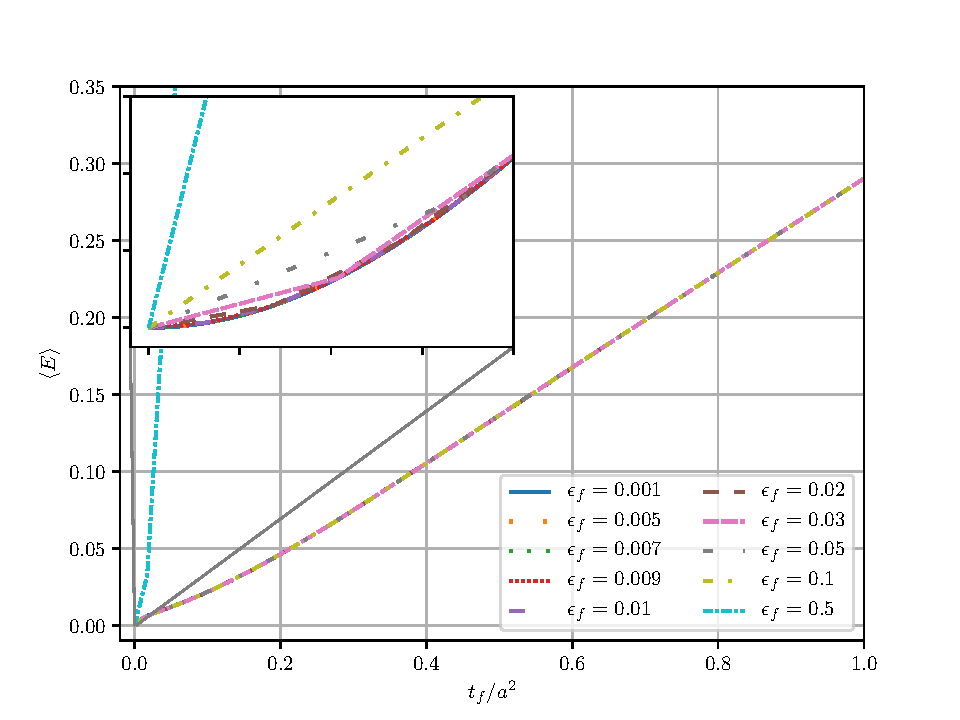
\includegraphics[trim={0.4cm 0.0cm 0.4cm 0.0cm},clip,scale=0.6]{../figures/flow-epsilon/energy}
\end{figure}}
\only<3->{The absolute difference between the smallest flow time $\epsilon_f=0.001$ and those shown previously.
\begin{figure}
    \centering
    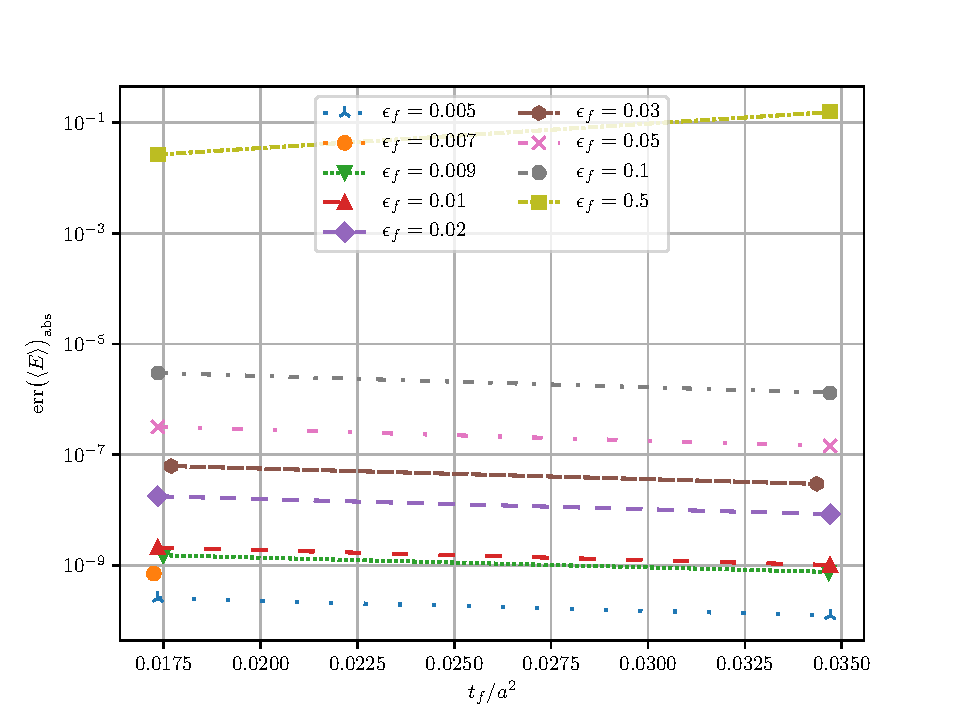
\includegraphics[trim={0.4cm 0.0cm 0.4cm 0.0cm},clip,scale=0.6]{../figures/flow-epsilon/energy_diff_absolute}
\end{figure}}
\note{
\begin{itemize}
    \item<1-> The values we will test the integrator against.
    \item<2-> The energy flowed for different the different $\epsilon_f$ values.
    \item<3-> The absolute difference between the smallest flow time $\epsilon_f=0.001$ and those listed in previous table.
    \item<3-> The reason for \textbf{only having two points} is due to the fact that we are only \textbf{comparing points} that are \textbf{close to each other in flow time}. If we were to have more points, we would have to double the number of flow time steps for the smallest lattices.
    \item<4-> An \textbf{example} of the flowing, can be seen by observing the \textbf{energy evolving over flow time}.
\end{itemize}}
\end{frame}

% \begin{frame}{Smearing the lattice: topological charge I}
% \begin{center}
%     \animategraphics[loop,controls,width=\linewidth,scale=0.6]{15}{../figures/latviz/topc_TE21/flowTime_TE21-}{0}{60}
% \end{center}
% \note{
% \begin{itemize}
%     \item Me and Giovanni Pederiva created a program for visualizing the gauge field.
%     \item Shows how the flow "removes noise" from the lattice, and only leaves large scale structures intact.
% \end{itemize}}
% \end{frame}

% \begin{frame}{Smearing the lattice: topological charge II}
% \begin{center}
%     \animategraphics[loop,controls,width=\linewidth,scale=0.7]{15}{../figures/latviz/topc_TE27/flowTime_TE27-}{0}{60}
% \end{center}
% \end{frame}

% \begin{frame}{Smearing the lattice: topological charge III}
% \begin{center}
%     \animategraphics[loop,controls,width=\linewidth,scale=0.7]{15}{../figures/latviz/topc_TF500/euclideanTime_tf500--}{0}{63}
% \end{center}
% \end{frame}


%%%%%%%%%%%%%%%%%%%%%%%%%%%%%%%%%%%%%%%%%%%%%%%%%%%%%%%%%%%%%%%%%%%%%%%%%%%%%%%%%%%%%%%%%%
%  ____                 _ _
% |  _ \ ___  ___ _   _| | |_ ___
% | |_) / _ \/ __| | | | | __/ __|
% |  _ <  __/\__ \ |_| | | |_\__ \
% |_| \_\___||___/\__,_|_|\__|___/
%%%%%%%%%%%%%%%%%%%%%%%%%%%%%%%%%%%%%%%%%%%%%%%%%%%%%%%%%%%%%%%%%%%%%%%%%%%%%%%%%%%%%%%%%%
\section{Results}

\begin{frame}{Ensembles}
% Include size and time
\begin{table}
    \centering
    \begin{tabular}{l r r r r r r r r}
        \toprule
        Ensemble & $\beta$ & $N$ & $N_T$ & $N_\mathrm{cfg}$ & $N_\mathrm{corr}$ & $N_\mathrm{up}$ & $\epsilon_\mathrm{flow}$ & Config. size$[$GB$]$ \\ 
        \midrule
        $A$ & 6.0 & 24 & 48 & 1000 & 600 & 30 & 0.01 & 0.356 \\
        $B$ & 6.1 & 28 & 56 & 1000 & 600 & 30 & 0.01 & 0.659 \\
        $C$ & 6.2 & 32 & 64 & 2000 & 600 & 30 & 0.01 & 1.125 \\
        $D_1$ & 6.45 & 32 & 32 & 1000 & 1600 & 30 & 0.02 & 0.563 \\
        $D_2$ & 6.45 & 48 & 96 & 250 & 1600 & 30 & 0.02 & 5.695 \\
        \bottomrule
    \end{tabular}
\end{table}
\note{
\begin{itemize}
    \item The main ensembles made for this thesis. 
    \item Every configuration was flown with $N_\mathrm{flow}=1000$ flow steps.
    \item We should also mention that we generated a few additional ensembles for investigating other aspects of the topological charge.
\end{itemize}
}
\end{frame}

\begin{frame}{The clover field strength definition}
\begin{figure}
    \centering
    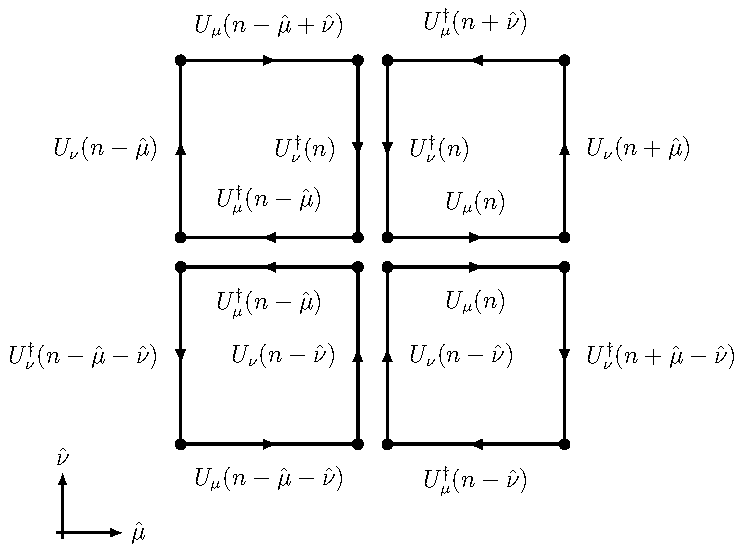
\includegraphics[scale=0.7]{../figures/illustrations/lqcd/clover/clover}
\end{figure}
\note{
\begin{itemize}
    \item We will use the clover field strength definition in gauge observables.
\end{itemize}
}
\end{frame}

\begin{frame}{Energy definition}
\onslide<1->{\begin{align*}
    E &= \frac{a^4}{2|\Lambda|} \sum_{n\in\Lambda}\sum_{\mu,\nu} \left(F^\mathrm{clov}_{\mu\nu}(n)\right)^2 \\
\end{align*}}
\onslide<2->{We can use this definition to set a scale $t_0$,
\begin{align*}
    \left\{t^2_f \expect{E(t)} \right\}_{t_f = t_{0}} = 0.3.
\end{align*}
}
\note{
\begin{itemize}
    \item We can use this definition to set a scale.
\end{itemize}
}
\end{frame}

\begin{frame}{Energy}
\begin{figure}
    \centering
    \includegraphics[trim={0.2cm 0.0cm 0.2cm 0.0cm},clip,scale=0.7]{../../LQCD/LatticeAnalyser/figures_b645_32xx4_full/data11/post_analysis/energy/post_analysis_energy_bootstrap_zoomed.pdf}
\end{figure}
\end{frame}

\begin{frame}{Scale setting \texorpdfstring{$t_0$}{t0}}
\only<1>{
\begin{table}
    \centering
    \begin{tabular}{l r r r r r r}
        \toprule
        Ensemble     & $t_0$[fm$^2$]   & $t_0/a^2$       & $t_0/r_0^2$     & $L/a$           & $L$ $[\fm]$        & $a$ $[\fm]$        \\ \midrule
        $A$          & $0.02780(2)$    & $3.20(3)$       & $0.11121(9)$    & $24$            & $2.235(9)$      & $0.0931(4)$     \\ 
        $B$          & $0.02769(2)$    & $4.43(4)$       & $0.11075(10)$   & $28$            & $2.214(10)$     & $0.0791(3)$     \\ 
        $C$          & $0.02775(2)$    & $6.01(6)$       & $0.11099(8)$    & $32$            & $2.17(1)$       & $0.0679(3)$     \\ 
        $D_1$        & $0.02779(5)$    & $12.2(1)$       & $0.1112(2)$     & $32$            & $1.530(9)$      & $0.0478(3)$     \\ 
        $D_2$        & $0.02794(9)$    & $12.2(1)$       & $0.1117(3)$     & $48$            & $2.29(1)$       & $0.0478(3)$     \\ 
        \bottomrule
    \end{tabular}
\end{table}}
\only<2-3>{
Continuum extrapolation using ensembles $A$, $B$, $C$, and $D_2$ gives $t_{0,\mathrm{cont}}/r_0^2 = 0.11087(50)$.
\begin{figure}
    \centering
    \includegraphics[trim={0.2cm 0.0cm 0.2cm 0.0cm},clip,scale=0.7]{../../LQCD/LatticeAnalyser/figures/data11/post_analysis/energy/post_analysis_extrapmethodbootstrap_t0reference_continuum_bootstrap.pdf}
\end{figure}
}
\only<4->{
    This matches the values retrieved by \citet{luscher_properties_2010}.
}
\note{
\begin{itemize}
    \item <1->Extrapolation results for $t_0$, where we retrieved the exact point of intersection between $t_f^2 \expect{E}$ and $0.3$ using $N_\mathrm{bs}=500$ bootstrap fits. Extrapolating to the continuum gives us $t_{0,\mathrm{cont}}/r_0^2 = 0.11087(50)$.
    \item <2->The continuum extrapolation $a\rightarrow 0$ for $t_0$ of the four ensembles $A$, $B$, $C$, and $D_2$.
    \item <3->$r_0=0.5$ fm.
\end{itemize}
}
\end{frame}

\begin{frame}{Scale setting \texorpdfstring{$w_0$}{w0}}
\only<1>{Can also set a scale using the derivative which offers more granularity for small flow times,
\begin{align*}
    &W(t)|_{t=w_0^2} = 0.3, \\
    &W(t) \equiv t_f \frac{\dd}{\dd t_f} \left\{t^2_f \expect{E}\right\}.
\end{align*}
}
\only<2->{
    
}
\end{frame}

\begin{frame}{Autocorrelation in the energy}
\end{frame}

\begin{frame}{Topological charge definition}
\begin{align*}
    Q = a^4 \sum_{n\in\Lambda} q(n),
\end{align*}
with the charge density given by
\begin{align*}
    q(n) = \frac{1}{32\pi^2} \epsilon_{\mu\nu\rho\sigma} \tr\left[F_{\mu\nu}(n)F_{\rho\sigma}(n)\right].
\end{align*}
\note{
\begin{itemize}
    \item We will use the clover field strength definition.
    \item Symmetries will allow us to reduce the effective number of clovers need to calculate from 24 to 6.
\end{itemize}
}
\end{frame}

\begin{frame}{Topological charge}
\end{frame}

\begin{frame}{Topological charge autocorrelation}
\end{frame}

\begin{frame}{Topological susceptibility}
\end{frame}

\begin{frame}{The fourth cumulant}
\end{frame}

\begin{frame}{The topological charge correlator}
\end{frame}

\begin{frame}{The effective glueball mass}
\end{frame}

%%%%%%%%%%%%%%%%%%%%%%%%%%%%%%%%%%%%%%%%%%%%%%%%%%%%%%%%%%%%%%%%%%%%%%%%%%%%%%%%%%%%%%%%%%
\section{Conclusion}
%%%%%%%%%%%%%%%%%%%%%%%%%%%%%%%%%%%%%%%%%%%%%%%%%%%%%%%%%%%%%%%%%%%%%%%%%%%%%%%%%%%%%%%%%%
\begin{frame}
\end{frame}

\begin{frame}
Questions?
\end{frame}

%%%%%%%%%%%%%%%%%%%%%%%% Disposition %%%%%%%%%%%%%%%%%%%%%%%%
% Introduction/overview of presentation: motivation, goal of thesis
% QCD: what is qcd, qcd to pure gauge(max 2 slides), topology quickstart
% LQCD: discretize lattice, links, introduce topological charge with clover, energy
% Flow: introduce gradient flow, motivate
% Latviz animation of Q in flow time and Euclidean time
% Results: energy scale setting, topological charge, distributions, why D1 and D2 differs, top.sus., N_F, eff.mass, 
% Conclusion: 
% Questions?
% Extra slides

\begin{frame}
\bibliography{bibliography/lib.bib}
\end{frame}

\end{document}